Im nachfolgenden Teil sollen die theoretischen Grundlagen erläutert werden die für das Verständis dieser Arbeit wichtig sind. Dabei bilden die Prinzipien der drahtlosen Datenübertragung das Fundament, auf dem alle weiteren technischen Konzepte aufbauen.
\label{kap:grundlagen}
\subsection{Drahtlose Datenübertragung}
\input{pages/sections/30_theoretische_grundlagen/drahtlose_datenübertragung.tex}
\subsubsection*{Frequenz und Bandbreite}
Die Frequenz beschreibt, wie oft sich ein periodisches Signal pro Sekunde wiederholt. Sie wird in Hertz (Hz) angegeben und ist eng mit der Wellenlänge $\lambda$ verknüpft. Diese lässt sich aus der Ausbreitungsgeschwindigkeit $c$ des Signals und der Frequenz $f$ über $\lambda = c / f$ berechnen. Höhere Frequenzen entsprechen kürzeren Wellenlängen und erfordern in der Regel kleinere Antennenabmessungen.

Die Bandbreite eines Kommunikationskanals bezeichnet den Frequenzbereich, innerhalb dessen ein Signal mit akzeptabler Qualität übertragen werden kann. Sie wird ebenfalls in Hertz angegeben und ist sowohl durch physikalische Eigenschaften des Übertragungsmediums als auch durch elektronische Komponenten begrenzt. Die Bandbreite bestimmt zusammen mit der Signalqualität die maximal mögliche Datenrate. In vielen Kanälen beträgt sie nur einen Bruchteil der Mittenfrequenz, typischerweise zwischen 1 \% und 10 \% des Trägerfrequenzbereichs. \autocite[S. 4]{proakisDigitalCommunications2008}

\subsubsection*{Schlüsselmetriken der Verbindungsqualität: RSSI, SNR und PDR}
\input{pages/sections/30_theoretische_grundlagen/schlüsselmetriken_rssi_snr_pdr.tex}
\subsection{LoRa und LoRaWAN}
Im Nachfolgenden soll die Funktechnologie auf der diese Arbeit aufbaut beschrieben werden. LoRa (Long Range) bildet dabei die Pysikalische schicht wärend LoraWAN (Long Range Wide Area Network) die Netzwerkschicht übernimmt. Die genaue aufteilung kann der Abbildung \ref{fig:lora-lorawan-osi} entnommen werden.

\begin{figure}[H]
\centering
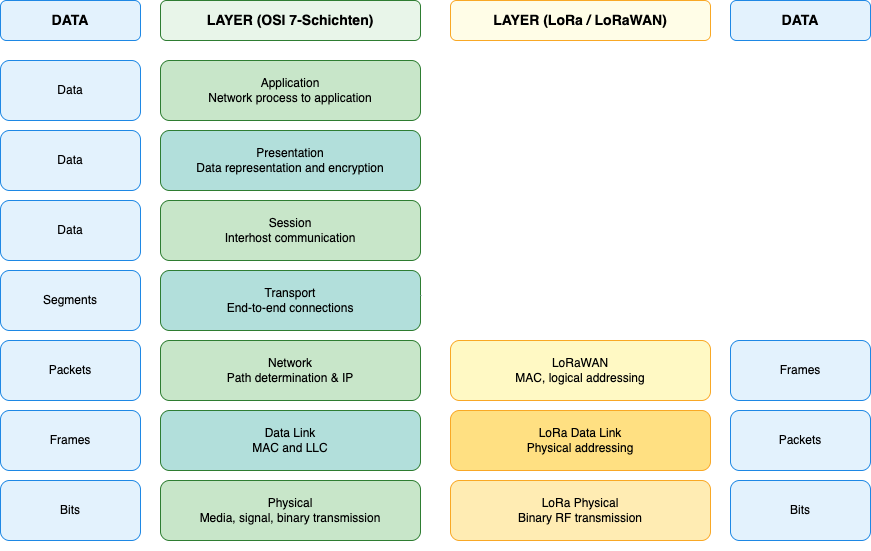
\includegraphics[scale=.4]{figures/diagrams/LoraWAN_OSI.png}
\caption{LoRa und LoRaWAN im OSI Schichtenmodell | Quelle: \ref{eckLoRaWANImDetail2019}}
\label{fig:lora-lorawan-osi}
\end{figure}

\subsubsection*{LoRa}
LoRa ist ein proprietäres und patentiertes drahtloses Übertragungsverfahren, das von der Semtech Corporation entwickelt wurde. Die Technologie arbeitet auf der physikalischen Schicht (Bitübertragungsschicht) und verwendet die Spread-Spectrum-Modulationstechnik \textit{Chirp Spread Spectrum} (CSS). CSS beinhaltet die Frequenzvariation eines Signals über die Zeit (Chirping). Ein „Upchirp“ ist eine Erhöhung der Frequenz von niedrig nach hoch, während ein „Downchirp“ eine Absenkung der Frequenz von hoch nach niedrig darstellt (siehe Abbildung \ref{fig:lora-chirp}). Diese Methode verteilt das Datensignal über ein breiteres Frequenzband, wodurch es robust gegenüber Rauschen und Interferenzen wird. 

\begin{figure}[H]
\centering
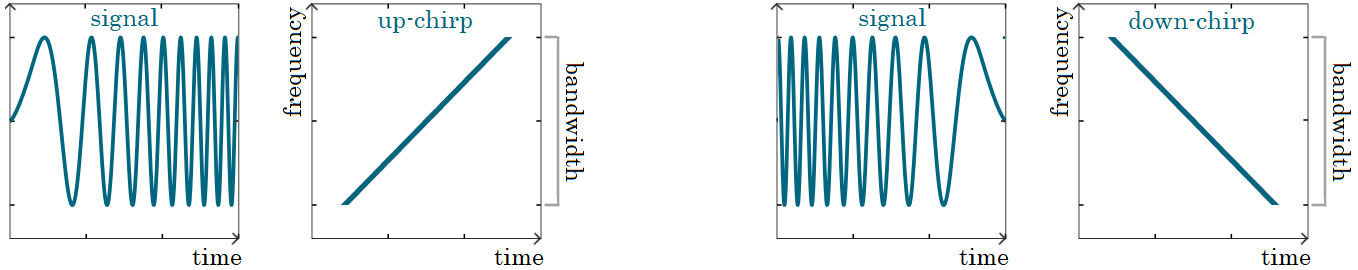
\includegraphics[scale=.4]{figures/asstes/lora-chirps.png}
\caption{LoRa Chirps | Quelle: \cite{tulkaLoRaSpreadingFactor}}
\label{fig:lora-chirp}
\end{figure}

Ein wesentlicher Vorteil von CSS gegenüber anderen Modulationstechniken, wie z.\,B. der in Abschnitt \ref{sec:drahtlosedatenübertragung} genannten FSK, ist die Fähigkeit, Signale selbst dann zu dekodieren, wenn sie unterhalb des Rauschpegels liegen. Dies wird durch die große Zeit-Bandbreite und die orthogonale Struktur der Chirp-Symbole ermöglicht.

\paragraph*{Spreading Factor} 
Der Spreading Factor (SF) beschreibt das Verhältnis zwischen der Chiprate und der Symbolrate. Wie aus Gleichung \ref{eq:spredigfactorbandwith} \cite[S.6]{rhode&schwarzCharacterizationLoRaDevices} ersichtlich, 
\begin{equation}
\label{eq:spredigfactorbandwith}
R_b = \frac{SF \cdot B}{2^{SF}} * \frac{4}{4 + CR},
\end{equation}
führt eine Erhöhung des SF zu einer größeren Reichweite, da das Signal robuster gegenüber Rauschen und Störungen wird. Gleichzeitig verringert sich jedoch die erzielbare Datenrate.


\paragraph*{Symbolstruktur und Datenübertragung}
Die Datenübertragung in LoRa erfolgt in Symbolen, die durch eine Folge von Chirps realisiert werden. Ein Symbolindex $s(nT_s)$ wird aus $SF$ (Spreading Factor) Bits gebildet (siehe Formel \ref{eq:lorasymbolindex}).
\begin{equation}
\label{eq:lorasymbolindex}
s(nT_s) = \sum_{h=0}^{SF-1} w_h(nT_s) \cdot 2^h, \quad s \in \{0,1,\dots,2^{SF}-1\}
\end{equation}
Jedes Symbol hat eine Dauer $T_s = 2^{SF} \cdot T$, wobei $T = \frac{1}{B}$ die Abtastperiode ist und $B$ die genutzte Bandbreite.

Das modulierte Signal für ein Symbol $s(nT_s)$ ist in Formel \ref{eq:loramoduliertesignal} zu sehen.
\begin{equation}
\label{eq:loramoduliertesignal}
c(nT_s + kT) = \frac{1}{\sqrt{2^{SF}}} e^{j 2\pi \frac{[(s(nT_s)+k) \bmod 2^{SF}] \cdot k}{2^{SF}}}, \quad k=0,\dots, 2^{SF}-1
\end{equation}
Dieses Signal stellt einen linearen Frequenzanstieg (Upchirp) dar, der um eine frequenzabhängige Startposition (abhängig vom Symbolwert $s$) verschoben ist. Ein Beispiel für diese Symbole kann Abbildung \ref{fig:lora-symbole} entnommen werden.

\begin{figure}[H]
\centering
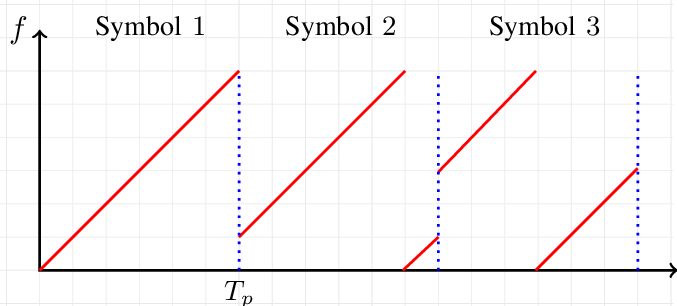
\includegraphics[scale=.4]{figures/asstes/n-LoRa-CSS-each-symbol-is-encoded-as-a-single-circularly-shifted-chirp-and-covers-the.png}
\caption{LoRa Symbole | Quelle: \cite{inproceedings}}
\label{fig:lora-symbole}
\end{figure}

\paragraph*{Erkennung unterhalb des Rauschpegels}
Die Fähigkeit, Signale unterhalb des Rauschpegels zu detektieren, basiert auf der \textit{Korrelation} zwischen empfangenem Signal und den orthogonalen Referenz-Chirps. Da LoRa-Symbole die gesamte Bandbreite $B$ abtasten, erfolgt eine Art \textit{Spektralspreizung}, die eine Energieintegration über die gesamte Symbolzeit ermöglicht. Der optimale Empfänger multipliziert das Empfangssignal mit einem Downchirp und führt anschließend eine diskrete Fourier-Transformation (DFT) durch. Das Maximum im Frequenzspektrum gibt den übertragenen Symbolindex an (siehe Formel \ref{eq:lorasymbolindex2}).
\begin{equation}
\label{eq:lorasymbolindex2}
\hat{s}(nT_s) = \arg \max_p \left| \sum_{k=0}^{2^{SF}-1} r(nT_s+kT) \cdot e^{-j 2\pi \frac{k^2}{2^{SF}}} \cdot e^{-j 2\pi \frac{p k}{2^{SF}}} \right|
\end{equation}
Durch die Integration über $T_s$ kann das Signal-Rausch-Verhältnis effektiv erhöht werden, wodurch eine Dekodierung auch unterhalb des thermischen Rauschpegels möglich ist. \autocite{tulkaLoRaSpreadingFactor, 8067462}


\subsubsection*{LoraWAN} 
\label{sec:lorawan}

LPWANs (Low Power Wide Area Networks) ermöglichen energieeffiziente Kommunikation über große Distanzen und gelten daher als eine Schlüsseltechnologie für das Internet der Dinge (IoT). LoRaWAN zählt zu den vielversprechendsten LPWAN-Technologien. Es bietet geringe Leistungsaufnahme, niedrige Kosten und große Reichweite, geht jedoch mit einer geringen Datenrate einher.

Das LoRaWAN-Kommunikationssystem besteht aus Endgeräten, Gateways, einem Netzwerkserver und den jeweiligen Anwendungen. Die Endgeräte kommunizieren über Funk mit den Gateways, welche die Daten an den Netzwerkserver weiterleiten. Von dort aus können dann andere Applikationen, meist über MQTT, die Daten auslesen und verwerten. 

\paragraph*{LoRaWAN-Geräteklassen}
Die LoRaWAN-Spezifikation definiert drei Endgeräteklassen \autocite{sornin2015lorawan}:

\begin{itemize}
    \item \textbf{Class A:} Für batteriebetriebene Geräte optimiert. Unterstützt bidirektionale Kommunikation mit einem Uplink-Fenster, gefolgt von zwei Downlink-Empfangsfenstern (RX1, RX2). Diese Funktionalität muss auf allen LoRaWAN-Geräten implementiert werden.
    
    \item \textbf{Class B:} Bietet zusätzlich geplante Empfangsfenster für vorhersagbare Downlinks. Geräte beginnen als Class A und können vom Server in Class B versetzt werden.
    
    \item \textbf{Class C:} Für netzbetriebene Geräte mit kontinuierlich offenem Empfangsfenster (RX2), was geringe Latenz ermöglicht. Diese Geräte verbrauchen mehr Energie im Vergleich zu anderen Geräteklassen.
\end{itemize}

\paragraph*{Leistungsmerkmale und Herausforderungen}
LoRaWAN kann durch Parameteroptimierung an unterschiedliche Anwendungen angepasst werden. Wichtige Designaspekte sind Skalierbarkeit, Durchsatz, Abdeckung, Energieeffizienz und geringe Kosten \cite{bor2017lora}. Herausforderungen bestehen insbesondere in:

\begin{itemize}
    \item \textbf{Skalierbarkeit:} Beeinflusst durch Faktoren wie verfügbare Kanäle, Spreizfaktor, Bandbreite und regulatorische Einschränkungen. In Europa steht für LoRa das Band von 863 MHz bis 870 MHz zur Verfügung, in Amerika von 902 MHz bis 928 MHz \autocite{FrequencyPlans}.
    
    \item \textbf{Energieeinsparung:} Durch die Adaptive Data Rate (ADR) oder eine optimierte Parameterwahl kann durch LoraWAN nochmals zusätzlich zu der ohnehin schon EStromspaarenden Lora-Technologie Energie eingespaart werden \autocite{kufakunesuSurveyAdaptiveData2020}.
    
    \item \textbf{Sicherheit:} Bei LoRaWAN spielt Sicherheit eine sehr wichtige Rolle, da Daten über Funk übertragen werden und damit leicht abgefangen werden könnten. Um das zu verhindern, werden Ende-zu-Ende-Schlüssel verwendet. Das bedeutet, dass Nachrichten bereits beim Gerät verschlüsselt werden und nur die dafür vorgesehenen Server diese wieder entschlüsseln können.  In der Praxis wird meist das Verfahren \emph{OTAA} (Over-The-Air Activation) eingesetzt. Dabei meldet sich das Gerät zunächst mit einem sogenannten Join-Vorgang am Netzwerk an. Hierfür gibt es einen eigenen \emph{Join Server}, der für die Schlüsselverwaltung zuständig ist. Nach erfolgreichem Join erhält das Gerät individuelle Sitzungsschlüssel, die für die eigentliche Kommunikation genutzt werden.  In öffentlichen Netzen ist es besonders wichtig, dass die verschiedenen Aufgaben klar voneinander getrennt sind. Der \emph{Join Server} übernimmt die Schlüsselverwaltung und den Beitritt, der \emph{Network Server} kümmert sich um die Organisation und Sicherheit des Funknetzes, und der \emph{Application Server} verarbeitet am Ende die entschlüsselten Anwendungsdaten. Diese Aufgabentrennung verhindert, dass Betreiber oder andere Parteien mehr Informationen einsehen können, als für sie notwendig ist. Außerdem wird dadurch eine sichere Verwaltung von Schlüsseln in Lieferketten und bei mehreren Nutzern (Multi-Tenant) ermöglicht, ohne dass ein Verlust der Schlüssel (\emph{Key Custody}) droht.  Damit die verschiedenen Server reibungslos zusammenarbeiten, wurden standardisierte Schnittstellen (Backend-Interfaces) entwickelt, die genau festlegen, wie die Kommunikation zwischen den Komponenten erfolgen soll. Untersuchungen zeigen zudem, dass die neuere Version \emph{LoRaWAN 1.1} deutliche Sicherheitsverbesserungen im Vergleich zur älteren Version 1.0 bietet. \autocite{butun2019security, LoRaWANBackendInterfaces11}

\end{itemize}

\paragraph*{Join-Mechanismus (OTAA)}
\label{sec:joinmechanissmus_otaa}
Bei der \emph{Over-The-Air Activation (OTAA)} meldet sich ein Endgerät bei dem Netzwerk an, indem es eine \emph{Join-Request}-Nachricht mit \emph{JoinEUI} (in LoRaWAN~1.0.x \emph{AppEUI}), \emph{DevEUI} und einem inkrementierenden \emph{DevNonce} sendet. Der \emph{DevNonce} ist ein 16-Bit-Wert und darf nie wiederverwendet werden. Dieser Wert muss in einem persistenten Speicher verwaltet werden. Der \emph{Join Server} prüft die Anfrage, generiert Sitzungsschlüssel und sendet eine verschlüsselte \emph{Join-Accept}-Nachricht zurück. In LoRaWAN~1.0.x werden dabei \emph{NwkSKey} und \emph{AppSKey} abgeleitet. In LoRaWAN~1.1 ersetzt ein erweitertes Schlüsselschema das \emph{NwkSKey} durch mehrere Netzwerkschlüssel (\emph{FNwkSIntKey}, \emph{SNwkSIntKey}, \emph{NwkSEncKey}). Der \emph{AppSKey} bleibt für Applikationsdaten bestehen. Eine erneute Anmeldung wird nur erforderlich, wenn Sitzungsschlüssel erneuert werden müssen. \autocite{thethingsnetworkJoin,techplayonJoin}

\paragraph*{Anwendungsgebiete}
LoRaWAN eignet sich für zahlreiche IoT-Szenarien, darunter smarte digitale Städte, smarte Messungen für zum Beispiel Pflanzen, smarter Parkverkehr indem Autofarern und Autofahrerinnen der weg zu einem freien Parkplatzt gezeigt wird oder intelligente Straßenbeleuchtung \autocite{BadenWuerttembergFoerdertLong2024}. Aufgrund der niedrigen Bitrate ist der Einsatz jedoch auf Anwendungen mit geringer Datenübertragungsrate beschränkt.

\paragraph*{Roaming, Peering und Interoperabilität}
LoRaWAN-Roaming erlaubt es, dass Endgeräte auch außerhalb des eigenen Netzwerks funktionieren können. Es gibt zwei Arten von Roaming:

\begin{itemize}
  \item \textbf{Passives Roaming:} Das Endgerät bleibt unter der Kontrolle seines Heimat-Netzservers (Serving NS), die Funkverbindung läuft aber über fremde Gateways und Netzserver (Forwarding NS). Diese leiten die Daten nur weiter, ohne die eigentliche Gerätesteuerung zu übernehmen.
  \item \textbf{Handover Roaming:} Hier übergibt der Heimat-Netzserver die Kontrolle an einen besuchten Netzserver (Serving NS). Dieser steuert dann das Endgerät aktiv, während der Heimat-NS im Hintergrund für die Schlüsselaushandlung und Verwaltung eingebunden bleibt.
\end{itemize}

Damit Roaming überhaupt funktioniert, müssen Netzbetreiber Peering- oder Roamingabkommen schließen. 
\emph{Packet Broker} bietet dazu ein globales Vermittlungsnetz, das den Austausch von Paketen zwischen verschiedenen Betreibern erleichtert. Ein Beispiel ist das offene Netz \texttt{The Things Network (TTN)} mit der \texttt{NetID~000013}. 

Kommerzielle Anbieter wie Senet setzen zusätzlich auf bilaterale Roaming-Vereinbarungen mit Partnernetzen, um ihre Abdeckung zu erweitern. \cite{LoRaWANBackendInterfaces11,PacketBroker,TTNNetID,SenetExt}


\paragraph*{Regulatorische Rahmenbedingungen (EU)}
In Europa wird das EU863–870-Band für LoRaWAN verwendet mit \emph{Duty-Cycle}-Grenzen je Subband (typisch 0{,}1–1\,\%\,/ 10\,\% im 869{,}4–869{,}65\,MHz-Subband) und Sendeleistungsgrenzen. Gerätekonfiguration und Kanalpläne folgen den \emph{LoRa Alliance Regional Parameters} (RP002), während die verbindlichen Funkparameter in \emph{ETSI EN~300~220} festgelegt sind. 
\autocite{RP002104, ETSIEN3002202025}
\subsection{Öffentliche LoraWAN Netzwerke}
\label{sec:ttn}

Öffentliche LoRaWAN-Netze stellen Konnektivität als gemeinschaftliche oder kommerzielle Infrastruktur bereit. Im Gegensatz zu privaten Netzen (unter eigener Kontrolle) unterscheiden sie sich durch \emph{Zugang} (offen vs. vertraglich), \emph{Kostenmodell} (kostenfrei/Fair-Use vs. verbrauchs- oder Service-Level-Agreement (SLA)-basiert \footnote{Ein SLA ist eine vertraglich festgelegte Leistungszusage zwischen Anbieter und Nutzer eines Dienstes (z.\,B. garantierte Verfügbarkeit, Reaktionszeit oder Durchsatz). \emph{SLA-basiert} bedeutet, dass das Netzwerk diese zugesicherten Leistungsmerkmale vertraglich garantiert.}), \emph{Peering/Roaming} sowie \emph{Betriebs- und Sicherheitsprozesse}. 
\autocite{LoRaWANBackendInterfaces11, RP002104, ETSIEN3002202025}

\subsubsection*{Abgrenzung und Kategorien}
In der Praxis zeigen sich drei Netzwerktypen:

\begin{enumerate}
  \item \textbf{Community-Netze} (z.\,B. The Things Network, TTN): offen, best-effort, Fair-Use, Enterprise-Plan.
  \item \textbf{Dezentrale Crowd-Netze} (z.\,B. Helium~IoT): von vielen Hotspot-Betreibern getragen, nutzungsbasierte Abrechnung.
  \item \textbf{Carrier/Neutral-Host} (z.\,B. Senet, Everynet): vertraglich, SLA/Peering, nur nationale Abdeckung.
\end{enumerate}

\subsubsection*{The Things Network (TTN)}
TTN ist ein globales Community-Netz auf Basis von \emph{The Things Stack}. Es bietet einen kostenfreien Zugang unter einer Fair-Use-Policy. Die Fair-Use-Policy limitiert in der kostenfreien Version u.\,a. die Uplink-Airtime pro Gerät und Tag. Genauer sind es „30 Sekunden Uplink-Airtime pro Tag (24 Stunden) und Gerät sowie maximal 10 Downlink-Nachrichten pro Tag (24 Stunden) und Gerät“ \autocite{DutyCycleTTN}. SLAs bestehen im Community-Netz nicht, jedoch bietet die Enterprise-Variante kommerzielle Zusagen. Das Netzwerk nutzt \emph{Packet Broker} als globales Rückrad zur sicheren Weiterleitung von Verkehr zwischen Netzen. Das TTN ist über die Community-Projekte TTN Mapper \& Packet-Broker-Mapper kartiert \autocite{TTNFairUse, PacketBroker, TTNMapperDoc}.  

Die Motivation zur Aufstellung eigener Gateways liegt im gemeinschaftlichen Charakter des Netzes: Durch zusätzliche Gateways wird die Netzabdeckung insgesamt verbessert, wovon wiederum alle Teilnehmer profitieren. Auch der Betreiber selbst erhält dadurch typischerweise eine stabilere Verbindung und bessere Abdeckung für seine eigenen Geräte. Jedoch ohne dass er dadurch mehr Nutzungsrechte erhält. TTN versteht sich damit als offenes, gemeinschaftsgetriebenes Infrastrukturprojekt, das vor allem durch den Nutzen der gemeinsamen Netzressourcen getragen wird.

\subsubsection*{Helium IoT}
Helium IoT ist ein globales LoRaWAN-Netzwerk, das von vielen unabhängigen Teilnehmern betrieben wird. Im Unterschied zu TTN ist die Nutzung nicht kostenlos, sondern erfolgt über sogenannte \emph{Data Credits (DC)}. Diese sind an den US-Dollar gebunden (fester Wert: 1\,DC = 0{,}00001\,USD) und können nur durch das \emph{Burning} von HNT-Token erzeugt werden. Dadurch wird ein direkter ökonomischer Anreiz geschaffen, der die Nachfrage nach Netzwerkressourcen mit dem Helium-Krypto-Token verbindet \autocite{HeliumDC}. 

Ein Uplink von 24~Byte entspricht einem Abrechnungsblock. Downlinks sind in der Regel kostenfrei, können jedoch durch zusätzliche Konfiguration zuverlässiger gestaltet werden. Dafür können Betreiber von LoRaWAN-Network-Servern (LNS) mehrere Gateway-Duplikate pro Uplink \enquote{einkaufen} (\emph{multibuy}), um die Wahrscheinlichkeit einer erfolgreichen Zustellung zu erhöhen \autocite{HeliumLNSAdv}.  

Neben der Nutzung führt das Modell von Helium auch zu einem finanziellen Anreiz für die Aufstellung von Gateways: Ähnlich wie bei anderen Kryptowährungen wird einem Betreiber eines Miners ein wirtschaftlicher Nutzen in Form von Token-Anteilen zugesichert. Betreiber erhalten durch die Bereitstellung eines Gateways und der damit verbundenen Netzwerkabdeckung Vergütungen in Form von HNT-Tokens. Die Höhe dieser Vergütung hängt dabei maßgeblich von der Erreichbarkeit benachbarter Gateways sowie von der Gateway-Dichte in der jeweiligen Region ab. Dieses Belohnungsmodell führte in der Vergangenheit zu einem schnellen und globalen Ausbau der Netzabdeckung, jedoch mit einer stark variierenden Qualität von Hardware und Installationsbedingungen.  

Während das Helium-Netz dadurch eine breite Abdeckung erreichen konnte, ist die resultierende Infrastruktur weniger einheitlich als bei klassischen Community-Netzen. Professionelle Gateways mit optimaler Standortwahl stehen oftmals neben kostengünstigen Geräten, die unter suboptimalen Bedingungen betrieben werden. Dies wirkt sich unmittelbar auf die Netzqualität und Zuverlässigkeit aus, verdeutlicht jedoch zugleich die Stärke des ökonomischen Anreizes als Treiber für den Netzausbau.

Die Netzabdeckung wird u.\,a. durch \emph{CoverageMap.net} vermessen, ein Service, der ursprünglich aus dem TTN Mapper-Projekt hervorgegangen ist \autocite{TTNMapperDoc}.


\subsubsection*{Carrier-/Neutral-Host-Netze (Beispiele: Senet, Everynet, Actility/ThingPark)}
Carrier- bzw. Neutral-Host-Netze bieten Konnektivität auf Basis von vertraglich zugesicherten Service-Level-Agreements (SLAs) an und greifen dabei teilweise auf überregionale Roaming-Abkommen zurück. 
Ein Beispiel ist \emph{Senet} in den USA, das durch Roaming-Abkommen eine erweiterte Netzabdeckung („Extended Coverage“) bereitstellt, unter anderem auch durch eine Integration mit Helium \autocite{SenetExt}. 
Das Unternehmen \emph{Everynet} betreibt Neutral-Host-Netze in mehreren Ländern und bietet zusätzlich Integrationen mit \emph{AWS IoT Core for LoRaWAN} an \autocite{AWSPublic}. 
\emph{Actility} mit seiner Plattform \emph{ThingPark} gilt als einer der verbreitetsten Anbieter in diesem Bereich und stellt sowohl Roaming-Funktionalitäten als auch hybride Szenarien für verschiedene Betreiber bereit \autocite{ETSIEN3002202025}.


\subsubsection*{Praktische Einordnung für diese Arbeit}
Für prototypische \emph{Tracking}-Workloads sind TTN (kostenfrei, Fair-Use) und Helium (breite Crowd-Abdeckung, DC-basiert) aufgrund ihrer großen Abdeckung und einfachen Anwendung naheliegend. 
Während TTN durch seine Community-getragene Struktur häufig qualitativ hochwertige Gateways bietet, die von technisch versierten Betreibern (z.\,B. Universitäten oder Kommunen) installiert werden, zeichnet sich Helium durch eine sehr große Anzahl an privat betriebenen Hotspots aus. 
Dies führt zu einer breiten globalen Abdeckung, jedoch erreichen die im Helium-Netz eingesetzten Gateways häufig nicht die Qualitätsstandards, wie sie im TTN-Umfeld üblich sind. Gründe hierfür sind unter anderem weniger optimale Installationsorte sowie der Einsatz kostengünstigerer Hardware, beispielsweise bei Antennen und Kabeln.
TTN eignet sich somit besonders für stabile Prototyping-Szenarien mit gut dokumentierten Tools und Community-Support, während Helium Vorteile bei einer schnellen globalen Skalierbarkeit bietet. 

\subsection{LoRaWAN Industrielle Anwendungsbereiche}
LoRaWAN (Long Range Wide Area Network) bietet durch seine Charakteristiken die in Abschnitt \ref{sec:lorawan} beschrieben viele Vorteile für industrielle Anwendungen. 

\paragraph*{Vorausschauende Instandhaltung} 
LoRaWAN ermöglicht eine zuverlässige und energiearme Übertragung von Zustandsdaten (z. B. Vibration, Temperatur) die für frühzeitige Wartungserkennung genutzt werden können. Besonders im Industrie-4.0-Umfeld lassen sich Sensoren schnell installieren, mit Legacy-Geräten koppeln und in Cloud-basierte Analyseplattformen integrieren, um Effizienz, Sicherheit und Zuverlässigkeit zu steigern \autocite{lorawansmartindustry}.

\paragraph*{Telemetrie und Alarmüberwachung}
LoRaWAN eignet sich für die gleichzeitige Übertragung von periodischen Telemetriedaten und seltenen Alarmmeldungen. Durch unterschiedliche Spreading-Factor-Zuweisung und gezielte Retransmission kann hohe Zuverlässigkeit für Alarme bei minimaler Verzögerung erreicht werden—ohne die reguläre Kommunikation zu beeinträchtigen \autocite{santos2020}.

\paragraph*{Umwelt- und Gefahrenüberwachung}
In industriellen Umgebungen mit Unfall- oder Störfallrisiko (z. B. toxische Gase) erlaubt ein LoRaWAN-System mit optimiertem Downlink-Control-Packet-Mechanismus zuverlässige, latenzarme Umweltdatenübermittlung zur schnellen Gefahrenabwehr \autocite{tamang2022}.

\subsection{Verwandte Arbeiten}
In diesem Abschnitt wird der aktuelle Forschungs- und Entwicklungsstand zu LoRaWAN im Kontext von Tracking-Systemen dargestellt. Ziel ist es, existierende Studien und Projekte zu analysieren, die sich mit der Leistungsfähigkeit, Energieeffizienz und Praxistauglichkeit von LoRaWAN im Bereich der globalen Güterüberwachung beschäftigen. 

\paragraph*{LoRaWAN im Vergleich zu anderen LPWAN-Technologien}
Mehrere Arbeiten vergleichen LoRaWAN mit alternativen LPWAN-Technologien wie Sigfox, NB-IoT und LTE-M. Studien zeigen, dass LoRaWAN insbesondere durch seine Flexibilität und die Verfügbarkeit von Community-Netzen (z.\,B. The Things Network genauer in Abschnitt \ref{sec:ttn} beschrieben) oft einfacher zu verwenden ist, während NB-IoT Vorteile in Netzstabilität und QoS bietet dafür aber auf Lizensierten Frequenzbändern arbeiten \cite{mekki2019overview, centenaro2016long,adelantado2017understanding}.  

\paragraph*{Leistungsfähigkeit und Reichweite}
Analysen der Reichweite von LoRaWAN zeigen, dass in urbanen Umgebungen typische Reichweiten von 2–5 km und in ländlichen Gebieten bis zu 15 km erreicht werden können \cite{augustin2016study, petajajarvi2017coverage}. Faktoren wie Bebauung, Antennenhöhe und Spreading Factor haben signifikanten Einfluss auf die Verbindungsqualität. 

\paragraph*{Energieeffizienz}
Für batteriebetriebene Endgeräte ist die Energiebilanz entscheidend. Arbeiten wie \cite{fialhoBatteryLifetimeEstimation2020, raza2017low,qiu2018survey} zeigen, dass LoRaWAN durch die Class-A-Architektur eine hohe Energieeffizienz erreicht, die Laufzeiten von mehreren Jahren bei typischen Sensordatenraten ermöglicht. Allerdings erfordert die Konfiguration des Duty-Cycles und der Sendeintervallen eine Balance zwischen Datenaktualität und Batterielaufzeit.

\paragraph*{Anwendungsgebiete in der Logistik}
LoRaWAN wird in zahlreichen Szenarien des IOTs eingesetzt, insbesondere in der Logistik für Güterverfolgung und Anwendungen in intelligenten Städten. Charakteristisch für die Anwendungsszenarien sind niedrige Datenraten, extrem geringer Energieverbrauch und lange Batterielaufzeiten, was für großflächige, wartungsarme Sensornetze wichtig ist. Im Bereich der Logistik werden vor allem Anwendungen wie die Überwachung von Transportgütern, Temperatur- oder Positionsdaten und allgemeine Güterverfolgung adressiert \cite{qiu2018survey}. Darüber hinaus betonen beide Studien die Bedeutung von Erweiterbarkeit und Zusammenarbeit zwischen verschiedenen Netzwerken, was durch Mechanismen wie Netzwechsel unterstützt werden kann \cite{raza2017low}.
